\begin{flushright}
    \textit{Лекция 18 (от 03.11)}
\end{flushright}
\theorem
При ДЛО пара симметричных точек относительно окружности или прямой $\gamma$
переходит в пару симметричных точек относительно образа $\gamma$ (окружности или
прямой).
\lemma
Точки $z$ и $z^*$ симметричны относительно окружности или прямой $\gamma$ тогда
и только тогда, когда любая окружность или прямая $\Gamma$: $z, z^* \in \Gamma$
перпендикулярна $\gamma$.
\pr (леммы)
\\
Рассмотрим случай, когда $\gamma$~--- окружность. 
\begin{itemize}
    \item Необходимость.
    \\
    Пусть $\Gamma$~--- также окружность, поскольку случай с прямой очевиден.
    \begin{figure}[h!]
        \centering
        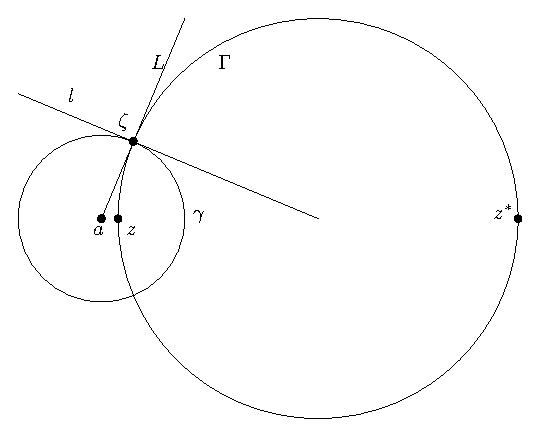
\includegraphics[scale=0.75]{neob.eps}
        \label{fig:23.1}
    \end{figure}
    Пусть $L$~--- касательная к $\Gamma$ из $a$, $\zeta \in L \cap \Gamma$.
    Тогда
    \begin{align*}
      & \left| a - \zeta \right|^2 = \left| a-z \right|\cdot \left| a-z^* \right| = R^2
    \end{align*}
    а значит, $\zeta \in \gamma$. Пусть $l$~--- касательная к $\Gamma$ в точке
    $\zeta$, $l \perp [a;\zeta] \Rightarrow l \perp L$.
    \item Достаточность.
    \begin{itemize}
        \item $\Gamma$~--- прямая, тогда $a \in \Gamma$, и значит, $z$ и $z^*$
        принадлежат одной полупрямой, исходящей из центра.
        \\
        Если точки лежат по разные стороны от центра, то построим окружность
        $\Gamma_1$ диаметром $zz^*$; тогда угол между $z$, точкой пересечения и
        $z^*$ равен $90^{\circ}$, а угол между $a$, точкой пересечения и центром
        окружности острый, т.~е. $L$ и $l$ не перпендикулярны).
            \begin{figure}[h!]
        \centering
        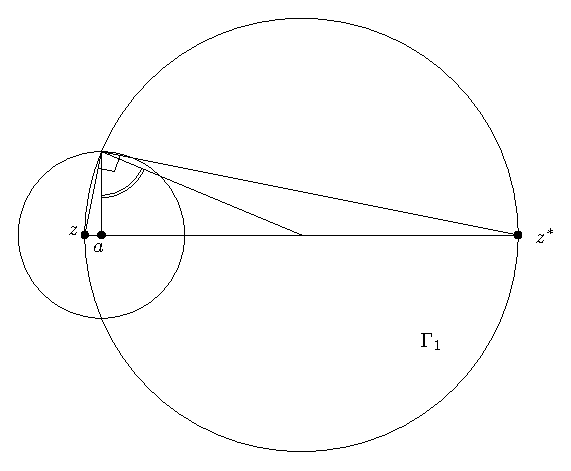
\includegraphics[scale=0.75]{dok.eps}
        \label{fig:23}
    \end{figure}
        \item $\Gamma$~--- окружность, тогда пусть $\zeta \in \Gamma \cap
        \gamma$, тогда
        \begin{align*}
          & \left| a - \zeta \right|^2 = \left| a-z \right|\cdot \left| a-z^* \right| = R^2
        \end{align*}
    \end{itemize}
\end{itemize}
\pr (теоремы)
$z$, $z^*$ симметричны относительно $\gamma$ (пусть окружности). Пусть $f$~---
ДЛО \eqref{(23.1)}, \eqref{(23.2)}. Пусть $w = f(z)$, $w^* = f(z^*)$, нужно
доказать, что они симметричны относительно $\tilde{\gamma} = f(\gamma)$.
\\
Рассмотрим $w$, $w^*$. Пусть $\tilde{\Gamma}$~--- любая окружность или прямая,
такая, что $w, w^* \in \tilde{\Gamma}$. Значит, по круговому свойству существует
окружность или прямая $\Gamma$: $\tilde{\Gamma} = f(\Gamma)$. По свойству
однолистности $z, z^* \in \Gamma$. Значит, по лемме $1$ $\gamma \perp \Gamma$.
Тогда, по свойству сохранения углов, $\tilde{\Gamma} \perp \tilde{\gamma}$. По
лемме $1$ тогда $w$ и $w^*$ симметричны относительно $\tilde{\Gamma}$.
\theorem
Множество ДЛО образует группу отображений относительно операции суперпозиции.
\pr
~
\begin{itemize}
    \item Очевидно, существует единичный элемент~--- тождественное отображение.
    \item У каждого ДЛО существует и единственно обратное ДЛО (см. теорему $1$).
    \item Суперпозиция ДЛО есть ДЛО. Действительно, пусть
    \begin{align*}
      & \zeta = \frac{a_1z+b_1}{c_1z+d_1}, \ w = \frac{a_2z+b_2}{c_2z+d_2}, \ a_1d_1 - c_1d_1 \neq 0, \ a_2d_2 - b_2c_2 \neq 0
    \end{align*}
    Положим
    \begin{align*}
      & z = \frac{z_1}{z_2}, \ \zeta = \frac{\zeta_1}{\zeta_2}, \ w = \frac{w_1}{w_2}
    \end{align*}
    Тогда
    \begin{align*}
      & \left( \begin{matrix}
              \zeta_1 \\
              \zeta_2
          \end{matrix} \right) = \left( \begin{matrix}
              a_1 & b_1 \\
              c_1 & d_1
          \end{matrix} \right) \cdot \left( \begin{matrix}
              z_1 \\
              z_2
          \end{matrix} \right), \ \left( \begin{matrix}
              w_1 \\
              w_2
          \end{matrix} \right) = \left( \begin{matrix}
              a_2 & b_2 \\
              c_2 & d_2
          \end{matrix} \right) \cdot \left( \begin{matrix}
              \zeta_1 \\
              \zeta_2
          \end{matrix} \right)
    \end{align*}
    \begin{align*}
      & \left( \begin{matrix}
              w_1 \\
              w_2
          \end{matrix} \right) = \left( \begin{matrix}
              a_2 & b_2 \\
              c_2 & d_2
          \end{matrix} \right) \cdot \left( \begin{matrix}
              a_1 & b_1 \\
              c_1 & d_1
          \end{matrix} \right) \cdot \left( \begin{matrix}
              z_1 \\
              z_2
          \end{matrix} \right)
    \end{align*}
    Получили невырожденное ДЛО.
\end{itemize}
\Example
Отобразить с помощью ДЛО области (см. рис.)
\begin{figure}[h!]
    \begin{minipage}[c]{0.45\textwidth}
        \centering
        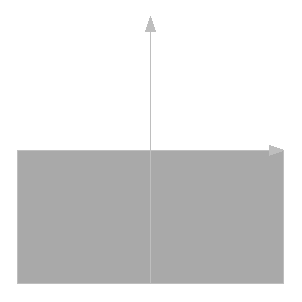
\includegraphics[scale=0.5]{half_plane.eps}
    \end{minipage}
    \begin{minipage}[c]{0.1\textwidth}
        \centering
        \LARGE{$\mapsto$}
    \end{minipage}
    \begin{minipage}[c]{0.45\textwidth}
        \centering
        
\includegraphics[scale=0.5]{round.eps}
    \end{minipage}
    \label{fig:23.2}
    \caption{$\Img z > 0 \mapsto \left| z \right| < 1$}
\end{figure}
\nonum
Возьмем любую $z_0: \ \Img z_0 > 0$. Пусть $z_0 \mapsto 0$, а $\ol{z_0} \mapsto
\infty$.
\\
Тогда
\begin{align*}
    & w = A\frac{z-z_0}{z-\ol{z_0}}
\end{align*}
Отыщем теперь $A$. Граница отображается на границу. Возьмем $x \in \RR$, она
должна отображаться на единичную окружность. Тогда
\begin{align*}
    & 1 = \abs{w} = \abs{A\frac{x-z_0}{x-\ol{z_0}}} = \left| A \right| \Rightarrow A = e^{i\alpha}
\end{align*}
Итак,
\begin{equation}\label{(23.6)}
    w = e^{i \alpha}\frac{z-z_0}{z-\ol{z_0}}
\end{equation}
\Example
Отобразить с помощью ДЛО области (см. рис.).
\\
\begin{figure}[h!]
    \begin{minipage}[c]{0.45\textwidth}
        \centering
        
\includegraphics[scale=0.5]{round.eps}
    \end{minipage}
    \begin{minipage}[c]{0.1\textwidth}
        \centering
        \LARGE{$\mapsto$}
    \end{minipage}
    \begin{minipage}[c]{0.45\textwidth}
        \centering
        
\includegraphics[scale=0.5]{round.eps}
    \end{minipage}
    \label{fig:23.3}
    \caption{$\left| z \right| < 1 \mapsto \left| z \right| < 1$}
\end{figure}
\nonum
Возьмем произвольную $z_0$ и отобразим ее в ноль; тогда симметричная $z_0^* =
\dst \frac{1}{\ol{z_0}}$ перейдет в $\infty$.
\\
Тогда
\begin{align*}
    & w = A\frac{z-z_0}{z-\dst \frac{1}{\ol{z_0}}} = \tilde{A}\frac{z-z_0}{1 - z\ol{z_0}}
\end{align*}
Граница перейдет в границу, а значит,
\begin{align*}
    & 1 = \abs{w} = \abs{\tilde{A}\frac{e^{i \varphi}-z_0}{1 - e^{i \varphi}\ol{z_0}}} = \abs{\tilde{A}\frac{e^{i \varphi}-z_0}{e^{-i \varphi}-\ol{z_0}}} = \abs{\tilde{A}}
\end{align*}
Итак,
\begin{equation}\label{(23.7)}
    w = e^{i \alpha}\frac{z-z_0}{1 - z\ol{z_0}}
\end{equation}
\Example
Отобразить с помощью ДЛО три различные точки $z_1, z_2, z_3$ в три точки $w_1,
w_2,w_3$.
\nonum
Заметим, что условиям удовлетворяет отображение вида
\begin{equation}\label{(23.8)}
    h(z) = \frac{z-z_1}{z-z_2} \cdot \frac{z_3-z_2}{z_3-z_1} = \frac{w-w_1}{w-w_2} \cdot \frac{w_3-w_2}{w_3-w_1} = g(w)
\end{equation}
\begin{align*}
  & w = f(z) = g^{-1}(h(z))
\end{align*}
Существование получено. Докажем единственность.
\\
Пусть для начала $f(z_k) = z_k$, тогда
\begin{align*}
  & \frac{az_k + b}{cz_k+d} = z_k
\end{align*}
\begin{align*}
  & cz^2_k + (d-a)z_k - b = 0
\end{align*}
Значит, поскольку квадратное уравнение имеет три решения, все его коэффициенты
равны нулю. Значит, $f(z) = z$.
\\
Пусть существуют $f_1(z)$, $f_2(z)$, причем $f_1(z_k) = f_2(z_k) = w_k$; тогда
$z_k = f_1^{-1}(f_2(z_k))$, тогда по групповому свойству $f_1^{-1}(z) =
f_2^{-1}(z)$, а значит, $f_1(z) = f_2(z)$.
\Example
Отобразить с помощью ДЛО области (см. рис.).
\\
\begin{figure}[h!]
    \begin{minipage}[c]{0.45\textwidth}
        \centering
        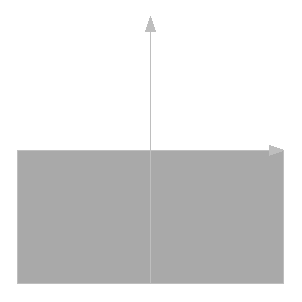
\includegraphics[scale=0.5]{half_plane.eps}
    \end{minipage}
    \begin{minipage}[c]{0.1\textwidth}
        \centering
        \LARGE{$\mapsto$}
    \end{minipage}
    \begin{minipage}[c]{0.45\textwidth}
        \centering
        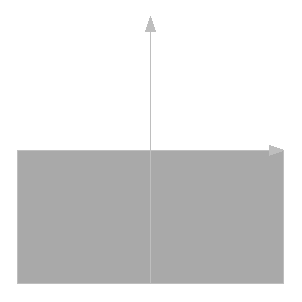
\includegraphics[scale=0.5]{half_plane.eps}
    \end{minipage}
    \label{fig:23.4}
    \caption{$\Img z > 0 \mapsto \Img z > 0$}
\end{figure}
\nonum
Пусть $x_1, x_2, x_3 \in \RR$, $x_1 < x_2 < x_3$, $u_1, u_2, u_3 \in \RR$, $u_1
< u_2 < u_3$, построим отображение $f(x_k) = u_k$. по примеру $3$ такое
отображение существует и единственно, границу оно переводит в границу. Из
свойства сохранения углов следует сохранение ориентации границы. Рассматривая
\eqref{(23.8)}, получаем все действительные  коэффициенты, т.~е. $a, b, c, d \in
\RR$, тогда $\forall x \in \RR \ \argm w'(x) = 0 \Rightarrow w'(x) > 0$, т.~е.
\begin{align*}
  & w'(x) = \frac{ad-cb}{(cx+d)^2} > 0 \Leftrightarrow ad-cb > 0
\end{align*}
Итак, необходимо и достаточно, чтобы все коэффициенты ДЛО были действительны,
причем $ad-cb > 0$.
\section{$\S 24.$ Конформные отображения элементарными функциями. Теорема Римама.}
Рассмотрим функции, обладающие локальной однолистностью.
\begin{center}
    \textbf{Степенная функция}
\end{center}
Фиксируем $t > 0$, рассмотрим область $G = \CC \setminus [0;+\infty)$. Пусть
\begin{align*}
  & w = \left| z \right|^t \exp(it \argt z), \ \argt z \in (0, 2 \pi)
\end{align*}
Функция регулярна при любом $t$. Действительно,
\begin{align*}
  & h(z) = \ln \left| z \right| + i \argt_0 z
\end{align*}
регулярна на этой области, а
\begin{align*}
  & w = \exp(t h(z))
\end{align*}
регулярна в этой области, как суперпозиция регулярных функций.
\\
Исследуем теперь однолистность. Рассмотрим
\begin{align*}
  & G_{0,\varphi_0} = \left\{ z \mid \left| z \right| > 0, \ \argt z \in (0; \varphi_0)\right\}
\end{align*}
\begin{align*}
  & l_{\varphi} = \left\{ z \mid z = r e^{i \varphi}, \ r > 0, \ \varphi \in (0, \varphi_0)\right\}
\end{align*}
Тогда
\begin{align*}
  & w(l_\varphi) = \left\{ w \mid w = \rho e^{i t \varphi}, \ \rho > 0 \right\}
\end{align*}
Тогда условие однолистности:
\begin{align*}
  & \begin{cases}
      0 < \varphi_0 < 2 \pi \\
      0 < t \varphi_0 < 2 \pi
  \end{cases}
\end{align*}
Значит, функция конформна на этой области.
\Example
$t = 2$, $w = z^2$.
\\
Условие однолистности: $\varphi_0 \in (0; \pi)$.
\begin{figure}[h!]
    \begin{minipage}[c]{0.45\textwidth}
        \centering
        
\includegraphics[scale=0.5]{half_round.eps}
    \end{minipage}
    \begin{minipage}[c]{0.1\textwidth}
        \centering
        \LARGE{$\mapsto$}
    \end{minipage}
    \begin{minipage}[c]{0.45\textwidth}
        \centering
        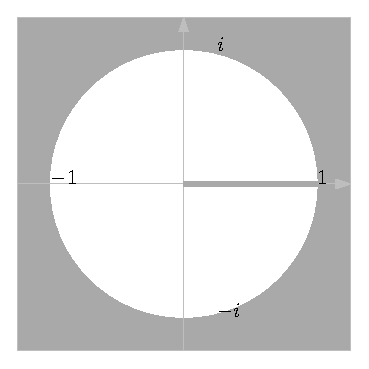
\includegraphics[scale=0.5]{cut_rnd.eps}
    \end{minipage}
    \label{fig:24.1}
\end{figure}
\\
Заметим, что данный полукруг содержится в $G_{0, \pi}$~--- области
однолистности, значит, функция будет однолистна.
\Example
$t = 2$, $w = z^2$.
\\
Условие однолистности: $\varphi_0 \in (0; \pi)$.
\begin{figure}[h!]
    \begin{minipage}[c]{0.45\textwidth}
        \centering
        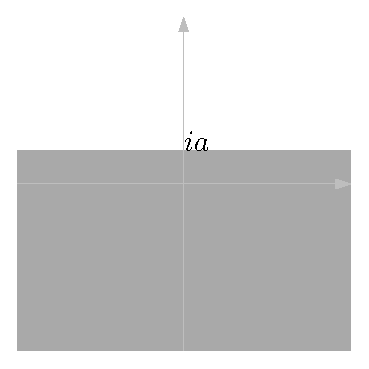
\includegraphics[scale=0.5]{top.eps}
    \end{minipage}
    \begin{minipage}[c]{0.1\textwidth}
        \centering
        \LARGE{$\mapsto$}
    \end{minipage}
    \begin{minipage}[c]{0.45\textwidth}
        \centering
        
\includegraphics[scale=0.5]{parabola.eps}
    \end{minipage}
    \label{fig:24.2}
\end{figure}
\\
Заметим, что данная полуплоскость содержится в $G_{0, \pi}$~--- области
однолистности, значит, функция будет однолистна. Зная, что граница переходит в
границу, отыщем $w(x+ia)$.
\begin{align*}
  & w(x+ia) = (x+ia)^2 = x^2 - a^2 + 2ixa
\end{align*}
\begin{align*}
  & \begin{cases}
      u = x^2 - a^2 \\
      v = 2xa
  \end{cases} \Rightarrow u  = \left( \frac{v}{2a} \right)^2 - a^2
\end{align*}
Поскольку $0$ не лежит в полуплоскости, искомая область будет внешностью
параболы.
\Example
$w = \left| z \right|^{\frac{1}{2}}\exp \left(\dst \frac{i}{2}\argt z\right)$.
\begin{figure}[h!]
    \begin{minipage}[c]{0.45\textwidth}
        \centering
        
\includegraphics[scale=0.5]{parabola.eps}
    \end{minipage}
    \begin{minipage}[c]{0.1\textwidth}
        \centering
        \LARGE{$\mapsto$}
    \end{minipage}
    \begin{minipage}[c]{0.45\textwidth}
        \centering
        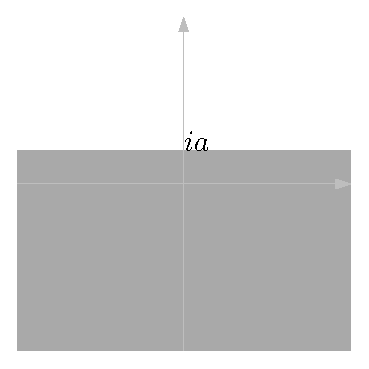
\includegraphics[scale=0.5]{top.eps}
    \end{minipage}
    \label{fig:24.3}
\end{figure}
Обратное к примеру $2$ отображение.
\begin{center}
    \textbf{Экспонента}
\end{center}
Всюду регулярна, но для однолистности необходимо, чтобы не было отличающихся на
$2 i \pi$ элементов (в силу периодичности).
\begin{figure}[h!]
    \centering
    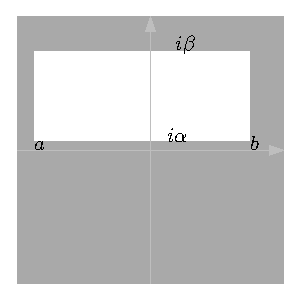
\includegraphics[scale=0.75]{odn_exp.eps}
    \label{fig:24.4}
    \caption{Область однолистности экспоненты}
\end{figure}
\begin{align*}
  & \begin{cases}
      -\infty \leq a \leq b \leq \infty \\
      0 \leq \beta - \alpha < 2 \pi
  \end{cases}
\end{align*}
\Example
\begin{figure}[h!]
    \begin{minipage}[c]{0.45\textwidth}
        \centering
        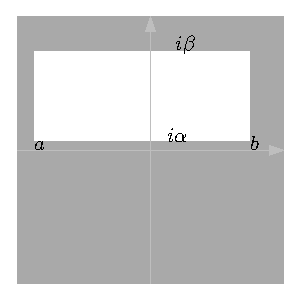
\includegraphics[scale=0.75]{odn_exp.eps}
    \end{minipage}
    \begin{minipage}[c]{0.1\textwidth}
        \centering
        \LARGE{$\mapsto$}
    \end{minipage}
    \begin{minipage}[c]{0.45\textwidth}
        \centering
        
\includegraphics[scale=0.5]{obraz_exp.eps}
    \end{minipage}
    \label{fig:24.5}
\end{figure}
Пусть $z = x+iy_0$, фиксированный $y_0 \in (\alpha,\beta)$. Тогда $\forall x \in
(a,b)$
\begin{align*}
  & f(z) = te^{iy_0}, \ t \in \left( e^{a}, e^{b} \right)
\end{align*}
\Example
~
\\
\begin{figure}[h!]
    \begin{minipage}[c]{0.45\textwidth}
        \centering
        
\includegraphics[scale=0.5]{polupolosa.eps}
    \end{minipage}
    \begin{minipage}[c]{0.1\textwidth}
        \centering
        \LARGE{$\mapsto$}
    \end{minipage}
    \begin{minipage}[c]{0.45\textwidth}
        \centering
        
\includegraphics[scale=0.5]{half_round.eps}
    \end{minipage}
    \label{fig:24.6}
    \caption{Перевод полуполосы в полуокружность.}
\end{figure}
Вертикальная черта переходит в полуокружность, верхняя граница~--- в отрезок
$[-1;0]$, нижняя граница~--- в отрезок $[0;1]$.
\Example
~
\\
\begin{figure}[h!]
    \begin{minipage}[c]{0.45\textwidth}
        \centering
        
\includegraphics[scale=0.5]{d_polupol.eps}
    \end{minipage}
    \begin{minipage}[c]{0.1\textwidth}
        \centering
        \LARGE{$\mapsto$}
    \end{minipage}
    \begin{minipage}[c]{0.45\textwidth}
        \centering
        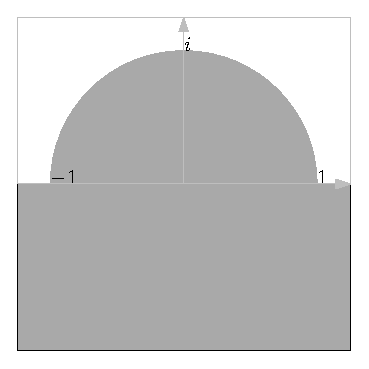
\includegraphics[scale=0.5]{out_rnd.eps}
    \end{minipage}
    \label{fig:24.7}
    \caption{Перевод полуполосы во внешность полуокружности.}
\end{figure}
